\documentclass[tikz,border=10pt]{standalone}
\usepackage{amsmath}
\usetikzlibrary{angles,quotes}
\begin{document}
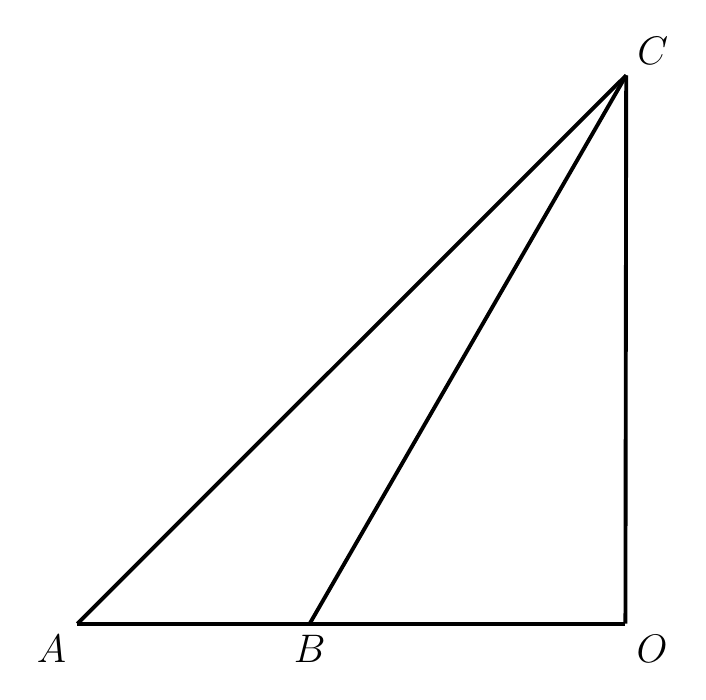
\begin{tikzpicture}[line width=1.4pt, line join=round]
\coordinate (A) at (-3.489,-3.464);
\coordinate (B) at (-0.538,-3.464);
\coordinate (C) at (3.482,3.501);
\coordinate (O) at (3.472,-3.464);




\draw (A) -- (B);
\draw (B) -- (O);
\draw (O) -- (C);
\draw (A) -- (C);
\draw (B) -- (C);




\node[below left] at (A) {\fontsize{14}{16.8}\selectfont $A$};
\node[below] at (B) {\fontsize{14}{16.8}\selectfont $B$};
\node[below right] at (O) {\fontsize{14}{16.8}\selectfont $O$};
\node[above right] at (C) {\fontsize{14}{16.8}\selectfont $C$};
\end{tikzpicture}
\end{document}